\section{Results}
\subsection{Part 1: Stopping Voltage and Wavelength}
\label{sec:results1}
Table \ref{tab:results1} lists all the measured stopping voltages for the light produced at each wavelength (uncertainty in wavelength was given as the bandwidth from the handout, and uncertainty in the stopping voltage is taken as the shown precision on the voltmeter) and the corresponding frequency using $f = \frac{c}{\lambda}$. The stopping voltage was plotted against the frequency in Figure \ref{fig:frequency_vs_voltage}. The data was fitted to a linear regression model, yielding the following relationship, where $V$ is the stopping voltage in $[V]$ and $f$ is the frequency in $[THz]$:
\begin{gather}
    V = (-1.329 \pm 0.056) + (0.00387 \pm 0.00009)f \\
    \chi^2 / \nu = 3.1 \times 10^{11} / 6 = 5.1 \times 10^{10}
\end{gather}
The residuals are small and random (Besides the IR light, which was not used in the regression calculation since it already reached 0 stopping voltage), which suggests a good fit. However, the $\chi^2$ value is atrociously large. This is due to the fact that we could calculate the voltage with very high precision, so any errors in our measurements were actually due to the wavelength uncertainties and not the voltages. Switching the dependent and independent variables gives a new $\chi^2$ value of 1.9, which is closer to the 6 degrees of freedom, supporting the fact that uncertainties are due to the frequency and not the voltage.

%Make table using results in data.tex for part 1
\begin{table}[H]
\centering
\caption{Stopping Voltage and Wavelength}
\label{tab:results1}
% Given Orange Red - 615 nm - 0.534304, format as |color|wavelength|voltage\pm0.0000001|
\begin{tabular}{|c|c|c|c|}
\hline
Color & Wavelength (nm) & Frequency (THz) & Stopping Voltage (V) \\ \hline
%Infrared - 935 nm - 0
Infrared & $935\pm10$ & $320\pm3$ & $0\pm0.000001$ \\ \hline
%Red - 640 nm - 0.508180:
Red & $640\pm10$ & $468\pm7$ & $0.508180 \pm 0.000001$ \\ \hline
%Orange Red - 615 nm - 0.534304:
Orange Red & $615\pm10$ & $487\pm8$ & $0.534304 \pm 0.000001$ \\ \hline
%Amber - 590 nm - 0.614265
Amber & $590\pm10$ & $508\pm9$ & $0.614265 \pm 0.000001$ \\ \hline
% Green - 535 nm - 0.870907
Green & $535\pm30$ & $560\pm31$ & $0.870907 \pm 0.000001$ \\ \hline
%Cyan - 505 nm - 0.965380
Cyan & $505\pm30$ & $594\pm35$ & $0.965380 \pm 0.000001$ \\ \hline
%Blue - 455 nm - 1.24025
Blue & $455\pm40$ & $659\pm58$ & $1.24025 \pm 0.00001$ \\ \hline
%UV - 390 nm - 1.63651
UV & $390\pm40$ & $769\pm79$ & $1.63651 \pm 0.00001$ \\ \hline
\end{tabular}
\end{table}
\begin{figure} 
    \centering
    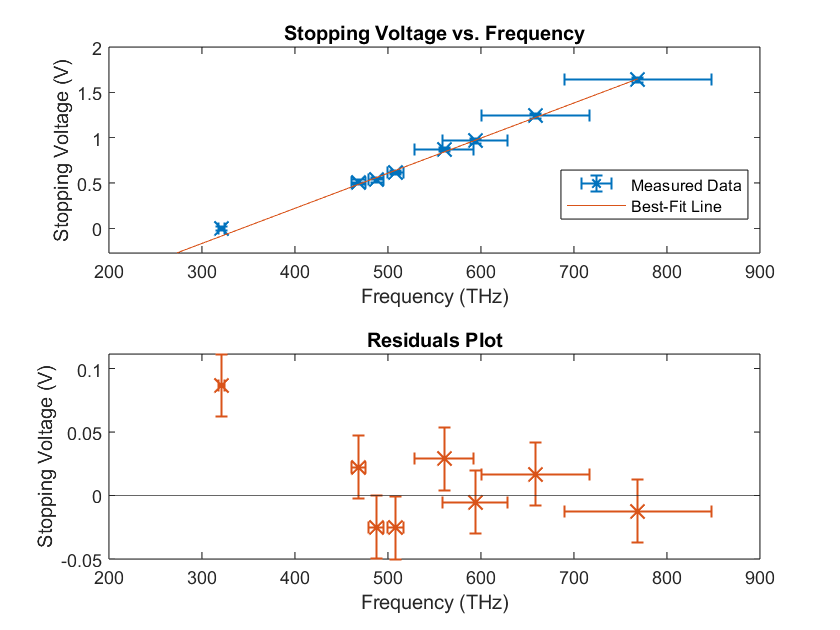
\includegraphics[width=0.8\textwidth]{Results/Frequency_vs_Stopping_Voltage.png}
    \caption{Stopping Voltage vs. Frequency. The IR light with 0V stopping voltage was not used in the fit, though it is still plotted with its residual}
    \label{fig:frequency_vs_voltage}
\end{figure}

Applying this fit to Equation \textbf{EDIT}, we can calculate planck's constant as:
\begin{gather*}
    h = (1.60217662 \times 10^{-19}~[C]) \cdot (0.00387 \pm 0.00009)~[V\cdot ps] \\
    = 6.21 \times 10^{-34} \pm 0.15^{-34} ~ [J\cdot s]
\end{gather*}

Comparing this to the true value of h at $6.62607015 \times 10^{-34}~[J\cdot s]$, we see that our value is more than 2 standard deviations away from the true value. This is not ideal, but we do have the number at the correct order of magnitude. The discrepancy is likely due to the uncertainty in wavelength, as the graph shows that at high frequencies, the uncertainty was quite significant relative to the data. 

Similarly, the stopping frequency is given by Equation \textbf{EDIT}:
\begin{gather*}
    f_0 = \frac{1.60217662 \times 10^{-19}~[C]}{6.21 \times 10^{-34} \pm 0.15^{-34} ~ [J\cdot s]}(1.329 \pm 0.056)~[V] = 343 \pm 16~[THz]
\end{gather*}
This represents the frequency below which the stopping voltage is 0, and the infrared light does indeed fall below this range and h as 0 stopping voltage, supporting this point.

Finally, we can thus calculate the work function for this phototube using Equation \textbf{EDIT}:
\begin{gather*}
    E_0 = (6.21 \times 10^{-34} \pm 0.15^{-34} ~ [J\cdot s]) \cdot (343 \pm 16~[THz]) = 2.1 \times 10^{-19} \pm 0.1^{-19} ~ [J] = 1.33 \pm 0.07 ~ [eV]
\end{gather*}

